\setupsectionbase
\section{Аналитическая часть}

	\par В данном разделе проводится анализ предметной области. 
	Рассматриваются базовые понятия цифрового представления аудиоданных,
	прикладные протоколы передачи потоковых данных, 
	рассматриваются виды форматов хранения аудиоданных.
	Проводится краткий обзор PCM формата хранения цифрового аудио.
	Дается анализ существующих средств воспроизведения аудиоданных в операционной системе iOS.

\subsection{Анализ предметной области}
	\par Воспроизведение потоковых аудиоданных на мобильных устройствах зависит от 
	протоколов потоковой передачи данных, форматов хранения аудиоданных, их обработки,
	а также от программных интерфейсов, предоставляемых разработчикам. 
	
	\par Зачастую используемые решения могут быть не универсальными, 
	а их выбор продиктован спецификой области применения и поставленными задачами.
	Так при построении системы транслирования радиоэфиров в реальном времени, можно принебречь качеством (разрешением звука) записи,
	а для системы прослушивания аудикниг, в которых важна дикция, задержка передачи данных не является важным критерием.

	\par Системным решением для воспроизведения потокового аудио на операционной системе iOS являются два
	комплекса программных интерфейсов: \newline AVFoundation \cite{avfoundation} и AudioToolbox \cite{audiotoolbox}. 
	Они являются частью системных компонентов и позволяют воспроизводить хранимые аудиофайлы в формате ACC, а также потоковое аудио, 
	транслируемое с помощью серверной части с использованием протоколов потоковой передачи данных HLS и HTTPS.
	Поддеживают высокие разрешение звука и частоту дискретизации.

	\par Рассмотрим сторонние решения, которые частично или полностью опираются на перечисленные комплексы программных интерфейсов, 
	а также решают задачи мультиплатформенности и поддержки несисистемных средств и аудиоформатов для воспроизведения аудиоданных в мобильном приложении.  

	\par VLCKit \cite{VLCKit} - библиотека для воспроизведения ACC файлов \cite{acc}, использующая программный интерфейс libVLC \cite{libVLC}, 
	реализованный для операционных систем: Linux, MacOS, Window, iOS, Android. 
	Данная библиотека поддерживает потоковое воспроизведение аудиоданных в ACC формате с низким разрешением звука, 
	с поддержкой протокола RTSP \cite{rtsp}.
	На текущий момент библитека не поддерживается для последних версий перечисленных операционных систем.
	
	\par SwiftAudioPlayer \cite{SwiftAudioPlayer} - программное обеспечение с открытым исходным кодом, 
	позволяющее воспроизводить потокое аудио в формате WAV \cite{wave-audio}
	с низкими разрешением звука и частотой дискретизации на операционной системе iOS 
	с использованием языка программирования Swift \cite{swift}.
	Поддерживает получение аудиоданных с помощью протокола потоковой передачи данных HLS \cite{hls}.
	За основу взят системный комплекс программных итерфейсов AVFoundation. 
	

\subsection{Цифровое представления аудиоданных}

	% \par Звук состоит из слышимых изменений давления воздуха. 
	% Звукозаписывающие устройства преобразуют изменение давления воздуха в переменное напряжение. 
	% Чтобы представить звук в цифровом виде, необходимо преобразовать это изменяющееся напряжение в ряд чисел, представляющих его амплитуду. 
	% Этот процесс известен как аналого-цифровое преобразование или дискретизация звука. 
	% Числа, выдаваемые аналого-цифровым преобразователем, в общем случае произвольны.

	% \par Изменение давления воздуха и, следовательно, соответствующее напряжение, создаваемое микрофоном, является непрерывным в двух измерениях.
	% То есть значения непрерывно изменяются, и они существуют в каждый момент времени.
	% Однако цифровая система, такая как компьютер, не может напрямую представлять непрерывный сигнал.
	% Вместо этого применяется ряд процессов для оцифровки звука:
	% \begin{itemize}
	% 	\item[---] Дискретизация --- преобразование сигнала в конечное множество дискретных моментов времени;
	% 	\item[---] Разрешение звука --- количество используемых дискретных уровней амплитуды сигнала;
	% 	\item[---] Квантование --- округление значения сигнала к одному из конечных дискретных уровней амплитуды. Обычно выражается в битах, то есть как логарифм по основанию 2 фактического числа;
	% \end{itemize} 
	% В результате вышеприведённых преобразований волна из своей непрерывной формы переходит в дискретизированную.
	
	\par Чтобы представить звук в цифровом виде, необходимо преобразовать это изменяющееся напряжение в ряд чисел, представляющих его амплитуду.
	Этот процесс известен как аналого-цифровое преобразование или дискретизация звука. 
	Числа, выдаваемые аналого-цифровым преобразователем, в общем случае произвольны.
	
	\par Цифровая система, такая как компьютер, не может напрямую представлять непрерывный сигнал.
	Вместо этого применяется ряд процессов для оцифровки звука:
	\begin{itemize}
		\item[---] Дискретизация --- преобразование сигнала в конечное множество дискретных моментов времени;
		\item[---] Разрешение звука --- количество используемых дискретных уровней амплитуды сигнала;
		\item[---] Квантование --- округление значения сигнала к одному из конечных дискретных уровней амплитуды. Обычно выражается в битах, то есть как логарифм по основанию 2 фактического числа;
	\end{itemize} 
	В результате вышеприведённых преобразований волна из своей непрерывной формы переходит в дискретизированную.
	На рис. \ref{fig:func} представлена непрерывная формы волны:

	\begin{figure}[!h]
		\center{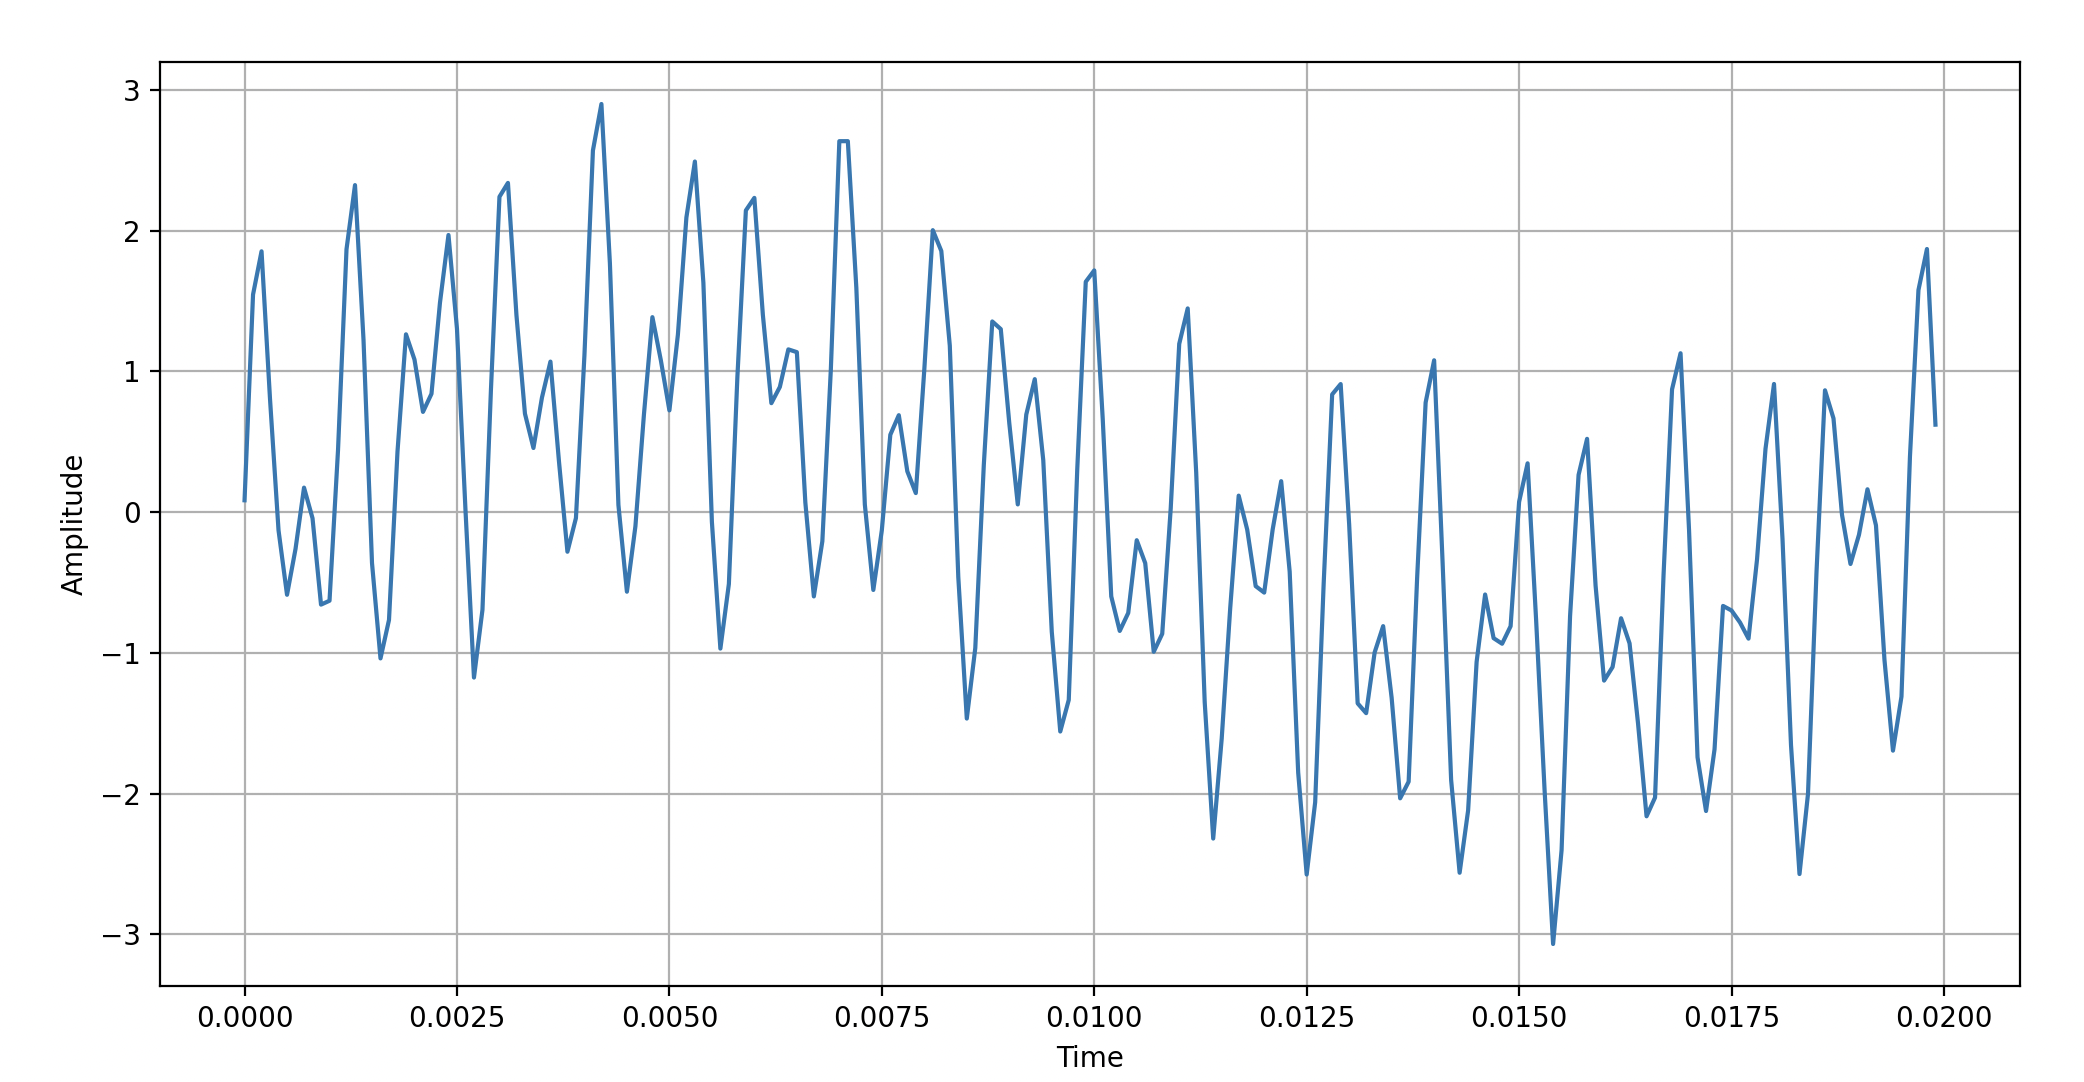
\includegraphics[scale=0.42]{img/func.png}}
		\caption{Непрерывная форма волны.}
		\label{fig:func}
	\end{figure}

	На рис. \ref{fig:dfunc} представлено наложение дискретных уровней, полученных в ходе дискретизация, на непрерывную форму волны:

	% \newpage
	\begin{figure}[!h]
		\center{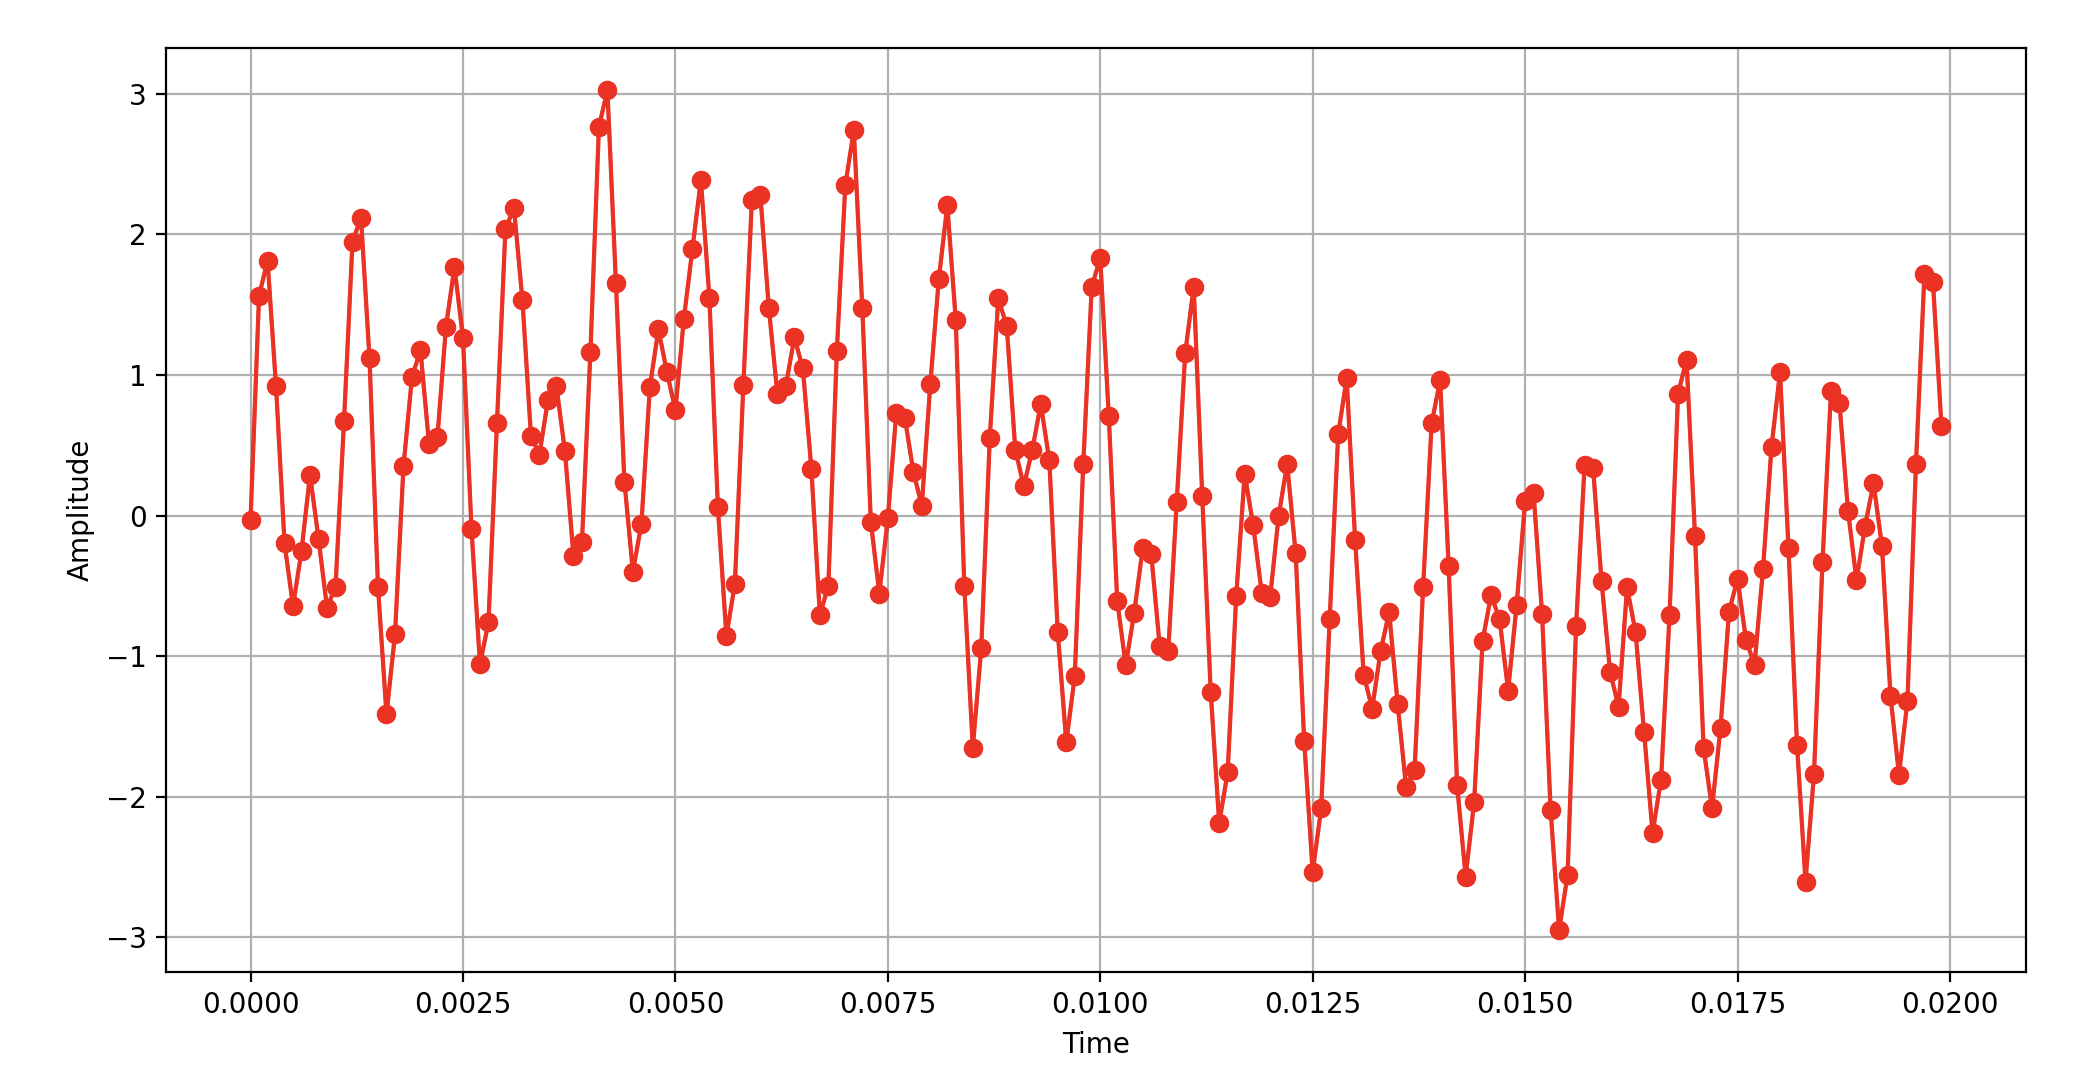
\includegraphics[scale=0.42]{img/dfunc.png}}
		\caption{Наложение дискретных уровней на непрерывную форму волны.}
		\label{fig:dfunc}
	\end{figure}

	\subsubsection*{Частота дискретизации}
	
		\par Частота дискретизации —-- это количество измерений амплитуды сигнала в секунду. Чем выше частота дискретизации, тем точнее дискретизированный сигнал будет представлять исходный сигнал. 

		\par Выбор частоты дискретизации определяется теоремой Котельникова о связи непрерывных и дискретных сигналов. 
		Данная теорема утверждает, что если максимальная частота спектра оригинального сигнала равна $f_{c}$,
		то при частоте дискретизации строго превышающей $2f_{c}$ возможно полностью восстановить исходный сигнал из дискретного вида.
		
		\par Другими словами, теорема Котельникова говорит о том, что непрерывный сигнал можно представить в виде интерполяционного ряда Фурье.
		Данное представление отображено формулой ниже:

		\begin{displaymath}
			% \label{eq:fur}
			\begin{cases}
				x(t) = \sum\limits^{\infty}_{k = -\infty}x(k\Delta)sinc[\cfrac{\pi}{\Delta}(t - k\Delta)], \\
				0 < \Delta \leq \cfrac{1}{2f_{c}},
			\end{cases}
		\end{displaymath}
		где $\Delta$ -- интервал дискретизации (сек.).
	
	\subsubsection*{Модуляция сигнала}
		\par Модуляция сигнала представляет собой процесс изменения параметров несущего сигнала (колебания) 
		с помощью модулирующего низкочастотного сигнала, где модулирующий сигнал хранит передаваемую информацию, 
		а несущий сигнал отвечает за передачу.

		Для цифрового представления дискретизированных аналоговых сигналов используются следующие методы модуляции:
		\begin{itemize}
			\item[---] импульсно-кодовая модуляция (PCM);
			\item[---] плотностно-импульсная модуляция (DSD);
		\end{itemize}

		\par Импульсно-кодовая модуляция \cite{PCM:DSD} является стандартной формой цифрового звука в вычислительных машинах
		и устройствах хранения данных. 
		В данном методе амплитуда аналогового сигнала дискретизируется через равные промежутки времени, 
		а затем квантуется. 
		Для обработки аудиоданных в PCM формате необходима поддержка PCM буфера, 
		который будет хранить пакеты аудиофайлов, полученных с помощью импульсно-кодовой модуляции.

		\par На рис. \ref{fig:PCMKvant} и \ref{fig:PCMBuffer} представлены квантование сигнала при импульсно-кодовой модуляции, 
		а также представление PCM буфера соответственно:

		% \newpage
		\begin{figure}[!h]
			\center{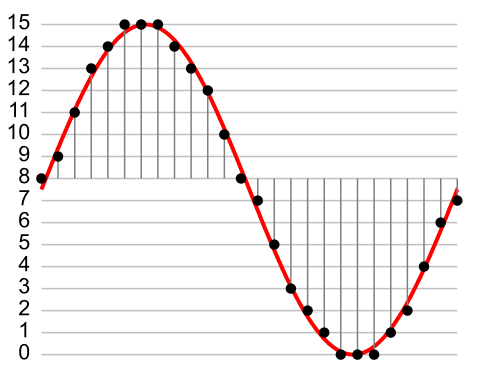
\includegraphics[scale=0.7]{img/pcm-kvant.png}}
			\caption{Квантование сигнала при импульсно-кодовой модуляции.}
			\label{fig:PCMKvant}
		\end{figure}

		\begin{figure}[!h]
			\center{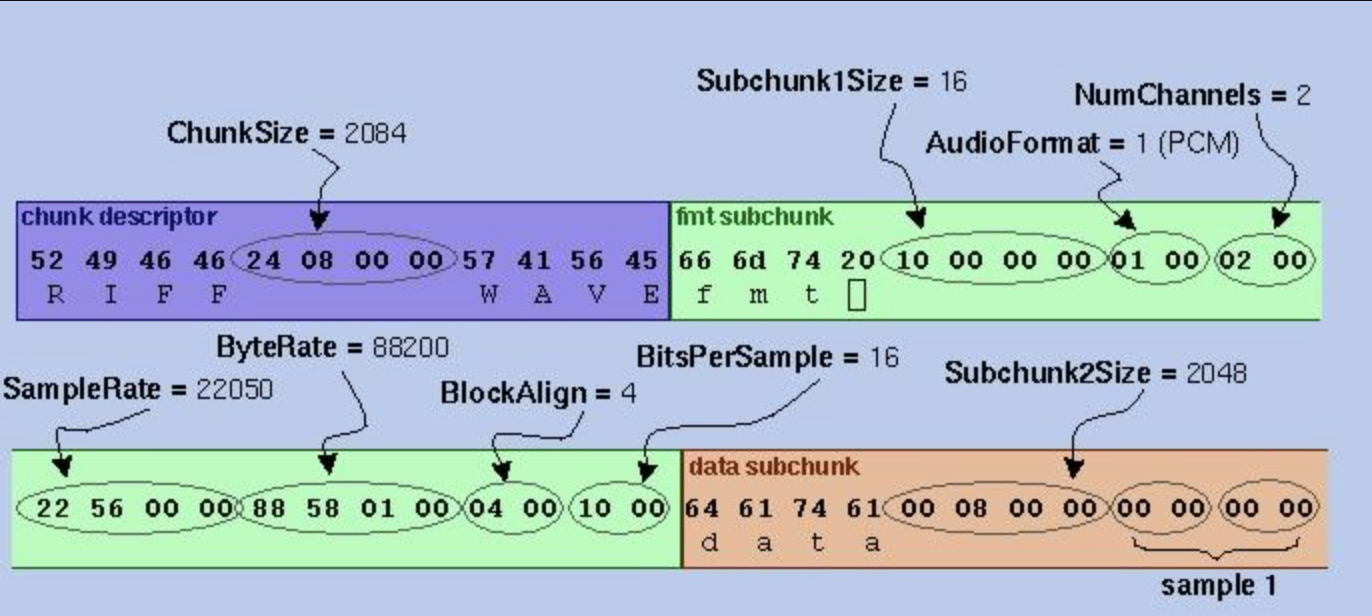
\includegraphics[scale=0.65]{img/pcm-buffer.png}}
			\caption{Представление PCM буфера.}
			\label{fig:PCMBuffer}
		\end{figure}

		\par DSD является однобитным аудиоформат, который получается в ходе \newline плотностно-импульсной модуляции \cite{PCM:DSD}, являющийся частным случаем сигма-дельта модуляции.
		Данный формат устарел и применялся для оптических носителей SACD. 
		Модуляция происходит при избыточной частоте дискретизации, а также при избыточном разрешении звука, 
		что позволяет уменьшить шум квантования. Он происходит при частоте сигнала, 
		амплитуда которого многократно превышает допустимое разрешение. 
		Для обработки аудиоданных в DSD формате необходимо использовать специальный DSD буфер, 
		хранящий однобитные пакеты аудиоданных.

		\par На рис. \ref{fig:DSMMod} представлено отличие плотностно-импульсной модуляции от импульсно-кодовой модуляции:
		\begin{figure}[!h]
			\center{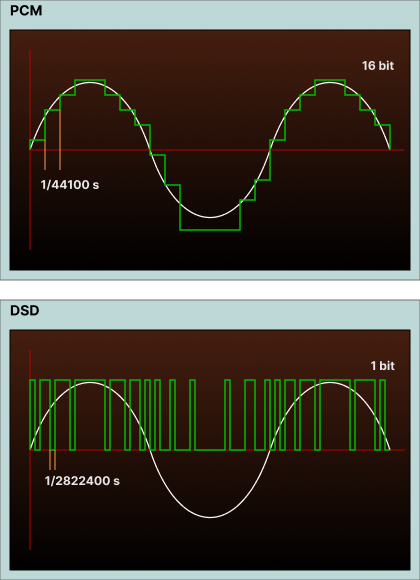
\includegraphics[scale=0.62]{img/dsm-mod.png}}
			\caption{Отличие плотностно-импульсной модуляции от импульсно-кодовой модуляции.}
			\label{fig:DSMMod}
		\end{figure}

		\par На текущий момент оцифровка звука в PCM формат 
		и обработка аудиоданных с помощью PCM буфера является наиболее распространенной.
		Большинство библиотек или программных интерфейсов, 
		ориентированных на воспроизведение аудиофайлов или потокового аудио, поддерживают работу с ним.
		
\subsection{Анализ форматов хранения аудиоданных}

	\par В общем случае аудиофайлы могут быть не сжаты, а также не иметь явного формата.
	Чаще всего аудиоданные обрабатывают для хранения по специальному формату, хранят в файле специального формата,
	представляющим <<заголовок>>, а также тело --- выборку целых чисел, характеризующих цифровой сигнал для воспроизведения аудио.

	\par Заголовок может содержать:
	\begin{itemize}
		\item[---] тип файла;
		\item[---] разрешение звука;
		\item[---] частота дискретизации;
		\item[---] информацию о сжатие, если таковое имеется;
		\item[---] количество байтов, следующих за заголовком;
		\item[---] ​​информацию о название и исполнителе;
	\end{itemize} 

	\subsubsection{Необработанные звуковые файлы}
		\par Звуковые файлы, которые не имеют заголовка, а содержат только числовую выборку, характеризующую цифровой сигнал, называются необработанными.
		Отсутствие явной информации о частоте дискретизации и разрешении позволяет использовать аудиоданные только по принятым соглашениям,
		которые принимаются между теми, кто упаковывает и использует данные аудиофайлы.

	\subsubsection{WAV (WAVE) формат}
		\par Для данного формата не применяется сжатие к битовому потоку, аудиозаписи хранятся с разными частотами дискретизации и битрейтами.  
		Однако WAV файлы имеют больший размер по сравнению с другими популярными форматами, такими как MP3, в которых используется сжатие с потерями для уменьшения размера файла при сохранении того же качества звука.
		Разрешение звука может быть как беззнаковым 8-битным, так и знаковым 16-битным (фрагменты дублируют информацию, найденную в других фрагментах). 
		Засчёт дубликатов блоков данных, характеризуют цифровой сигнал в конкретный момент времени, обработка информации может занять дополнительное время.
		
		\par Заголовок файла содержит:
		\begin{itemize}
			\item[---] размер файла в байтах;
			\item[---] длину блока данных;
			\item[---] количество аудиоканалов;
			\item[---] битрейт;
			\item[---] частота дискретизации;
		\end{itemize}

	\subsubsection{MP4 формат}
		\par MP4 \cite{mp4} —-- это международный стандарт кодирования аудиовизуальных материалов, 
		из-за высокой степени сжатия, результирующие файлы имеют меньший размер с почти полным сохранением исходного качества.
		Данные в файле MP4 разделены на два раздела, первый из которых содержит мультимедийные данные, а второй содержит метаданные.
		Структуры в MP4 обычно называются атомами или блоками. Минимальный размер атома составляет 8 байт (первые 4 байта определяют размер, а следующие 4 байта определяют тип).

		\par Первый раздел содержит следующую информаию:
		\begin{itemize}
			\item[---] таблица выборок значений цифрового сигнала в момент времени;
			\item[---] заголовок аудиоданных, содержащий частоты дискретизаии (до 48 кГц) и разрешение звука;
			\item[---] количество аудиоканалов;
			\item[---] битрейт;
		\end{itemize}

		\par Второй раздел содержит следующую информаию:
		\begin{itemize}
			\item[---] дескриптор файла;
			\item[---] информацию о сжатии;
		\end{itemize}

	
	\subsubsection{MP3 формат}
		\par Файл MP3 \cite{mp3} состоит из фреймов, каждый из которых состоит из заголовка и блока данных. 
		Фреймы не являются независимыми и обычно не могут быть извлечены на произвольных границах переходов фреймов. 
		Блоки данных файла содержат информацию об аудио с точки зрения частот и амплитуд. 
		Заголовок идентифицирует начало допустимого кадра. 
		Затем следуют 3 бита, где первый бит показывает, что это стандарт MPEG, а оставшиеся 2 бита показывают, что используется уровень MPEG-1 Audio Layer \cite{mpeg}. 
		После этого значения будут различаться в зависимости от содержимого конкретного аудиофайла.

		\par Заголовок фрейма содержит следующую информацию:
		\begin{itemize}
			\item[---] информация о переходе на текщий фрейм;
			\item[---] идентификатор версии MPEG Audio;
			\item[---] описание фрейма;
			\item[---] бит, который показывает, что фрейм зашифрован;
			\item[---] битрейт;
			\item[---] частота дискретизации (от 8 кГц до 48 кГц);
			\item[---] приватный ключ шифрования;
		\end{itemize}
	
	\subsubsection{AAC формат}
		\par AAC (Advanced Audio Coding) относится к стандарту цифрового кодирования звука, который представляет аудиофайлы на основе сжатия звука с потерями. 
		Он был запущен как преемник формата файла MP3 с учетом того, что у сторонних разработчиков возникли проблемы с реализацией новых идей в процессе кодирования, основанных на развитии методов сжатия данных. 
		AAC обеспечивает лучшее качество звука по сравнению с MP3 при той же скорости передачи данных. 
		Основные различия между AAC и MP3 с точки зрения улучшений заключаются в поддержке более широкого диапазона и частот дискретизации (от 8 кГц до 96 кГц).
		Разбиение по фреймам и содержание заголовка фрейма идентичны с MP3 форматом.
		
	\subsubsection{Сравнение форматов хранения аудиоданных}
		\par Сравнение рассмотренных форматов хранения аудиоданных рассмотрены в табл. \ref{tab:comparsion}. 
		Обозначения:
		\begin{itemize}
			\item[---] 1 --- поддержка частоты дискретизации более 48 кГц;
			\item[---] 2 --- наличие заголовка с метаинформацией;
			\item[---] 3 --- поддержка сжатия данных;
			\item[---] 4 --- фрагментация данных цифрового сигнала;
		\end{itemize}
		\begin{table}[hbtp]
			\caption{Сравнение форматов хранения аудиоданных}
			\centering
			\label{tab:comparsion}
			\begin{tabular}{|l|l|l|l|l|}
				\hline
				\textbf{Формат} & \textbf{1} & \textbf{2} & \textbf{3} & \textbf{4}   \\ \hline
				\text{WAV} & \textbf{+} & -          & -          &   -        \\ \hline
				\text{MP3} &   -        & \textbf{+} & \textbf{+} & \textbf{+} \\ \hline
				\text{MP4} &   -        & \textbf{+} & \textbf{+} & -          \\ \hline
				\text{ACC} & \textbf{+} & \textbf{+} & \textbf{+} & \textbf{+} \\ \hline
			\end{tabular}%
		\end{table}

		\par По результатам сравнения можно сделать вывод, что наиболее оптимальными форматами хранения аудиоданных являются ACC и MP3.
		Принципиальное отличие заключается в диапазоне поддерживаемых частот дискретизации. 
		При требовании поддержки частоты дискретизации до 48 кГц форматы равноэффективны, но при необходимости в поддержке частоты до 96 кГц,
		необходимо использовать формат ACC.
		Следует отметить, что формат WAV подходит в случае заранее принятых стандартов звукозаписи,
		при которых метаданные, хранящиеся в заголовках других форматов, будут известны. 

\subsection{Анализ протоколов передачи потоковых данных}

	\par Для передачи данных при стриминге необходимо использовать прикладные протоколы передачи данных,
	сжимающие данные для быстрой транспортировки, а также форматирующие данные в специальный формат.

	\subsubsection{HTTP/HTTPS}
		
	\par HTTP \cite{http} --- протокол прикладного уровня для передачи данных в формате гипертекста, 
	использующий протокол транспортного уровня TCP \cite{tcp}.
	Передача данных осуществляется в виде сегментов (пакетов) данных. 
	Гарантируется, что запрошенные пакеты данных будут доставлены и с необходимым порядком пакетов.
	Изначально при помощи HTTP протокола можно передавать данные только в формате гипертекста (HTML), 
	но для потоковой передачи данных можно настроить специальный механизм HTTP Long Polling.

	\par При потоковой передаче данных HTTP сервер настроен на удержание определенного запроса от клиента (HTTP Push). 
	Сервер сохраняет соединение с клиентом открытым и отправляет обновления относящиеся к запросу при доступности.
	В данном подходе отсутствует необходимость в постоянном запросе к серверу, 
	т.е. клиент отправляет единственный запрос на соединение, а также единственный запрос на разрыв соединения.

	В запросе, для установки постоянного соединения между клиентом и серверов, 
	необходимо передать заголовок $Transfer Encoding: chunked$. Это позволит определить на серверной стороне, 
	что передача данных должна проводиться с помощью HTTP Push.
	На рис. \ref{fig:http-push} представлена схема передачи данных с сервера на клиент с помощью HTTP Push.

	\begin{figure}[!h]
		\center{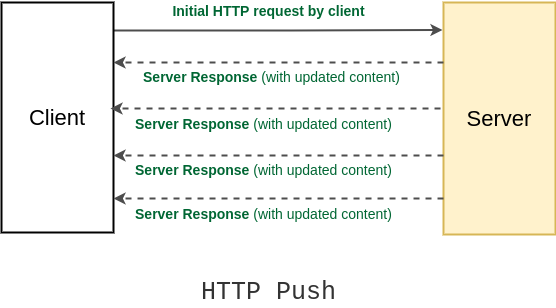
\includegraphics[scale=0.52]{img/Http-push.png}}
		\caption{Cхема передачи данных с сервера на клиент с помощью HTTP Push.}
		\label{fig:http-push}
	\end{figure}

	Следует отметить, что использование протокола HTTP для передачи потоковых аудиоданных является наиболее распространённым.
	При передаче пакетов аудиоданных придерживаются следующих правил:
	\begin{itemize}[leftmargin=1.6\parindent]
		\item[---] первые пакеты хранят данные относящиеся к метаинформации (заголовку) передаваемого аудиофайла;
		\item[---] остальные пакеты хранят информацию о звуковом сигнале;
	\end{itemize}
	
	\subsubsection{HLS (HTTP Live Streaming)}

		\par HLS --- это протокол потоковой передачи, который набирает всё большую популярность. 
		Данный протокол создан на основе протокола прикладного уровня HTTP, использующий протокол транспортного уровня TCP.
		Концептуально HTTP Live Streaming состоит из трех частей:
		\begin{itemize}[leftmargin=1.6\parindent]
			\item[---] серверный компонент;
			\item[---] компонент доставки;
			\item[---] клиентское программное обеспечение.
		\end{itemize}

		\par В классической конфигурации аппаратный кодировщик принимает на вход аудиофайл. 
		Происходит кодировка аудио в ACС формат, 
		затем программный сегментатор разбивает поток на серии коротких медиафайлов, размещающихся на сервере. 
		Сегментатор создает и поддерживает файл-индекс, содержащий список медиафайлов. 
		Клиент считывает индекс, затем запрашивает перечисленные файлы по порядку и отображает их без остановок, разрывов между сегментами.
		На рис. \ref{fig:hls} изображена схема принципа работы протокола HLS.

		\begin{figure}[!h]
			\center{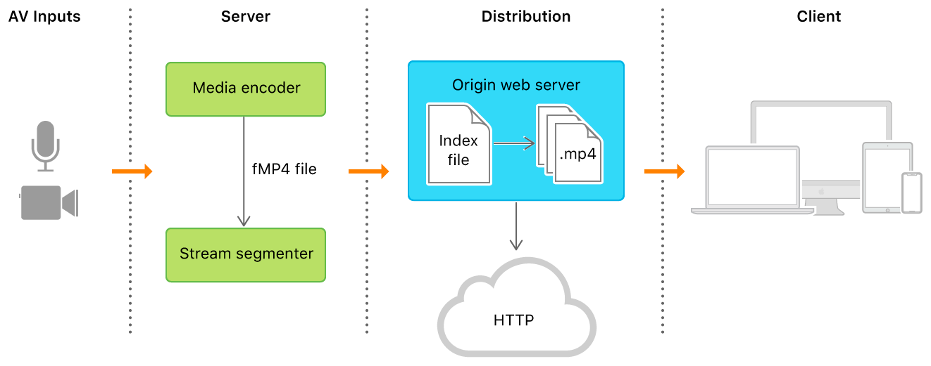
\includegraphics[scale=0.8]{img/hls.png}}
			\caption{Схема принципа работы протокола HLS.}
			\label{fig:hls}
		\end{figure}

		\par К достоинствам данного протокола можно отнести:
		\begin{itemize}[leftmargin=1.6\parindent]
			\item[---] сегментацая и индексация потка файлов, полученных в результате работы сегментатора;
			\item[---] поддержка ACC формата, что позволяет передавать аудиоданные с частотой дискретизации от 8 до 96 кГц;
			\item[---] гарантированная последовательная передачи пакетов без потерь;
		\end{itemize}

		\par К недостаткам данного протокола можно отнести:
		\begin{itemize}[leftmargin=1.6\parindent]
			\item[---] предварительная обработка исходного файла, которая заключается в разбиении и сжатии на подфайлы специального формата;
			\item[---] сильная задержка при передаче данных, которая не позволяет транслировать данные в режиме реального времени;
		\end{itemize}

	\subsubsection{Low-Latency HLS}

		\par Low-Latency HLS \cite{hls-ll} позволяет передавать медиа файлы на параллельных каналах, с помощью разделения медиафайлов на большее количество маленьких файлов CMAF Chunks. 
		Эти файлы называются частичными сегментами HLS. 
		Т.к. каждый частичный сегмент имеет меньшую длительность, он может быть упакован, передан или добавлен быстрее чем его родительский сегмент.
		Пока стандартный медиасегмент может быть длительностью 6 секунд каждый, частичный сегмент может быть до 1 секунды.

		\par Ускорение передачи данных достигается с помощью усложнения процесса предварительной обработки файла. 
		Происходит дробление подфайлов, полученных сегментатором, на частичные сегменты. 
		Создаётся список контекста сегментов, которые находятся в очереди на отправку данных.
		Параллельно происходит фильтрация списка, которая отбрасывает сегменты, которые считаются незначительными.

		\par По сравнению с стандартной организацией HLS, данный протокол обеспечивает более быструю передачу пакетов, 
		но требует дополнительной фильтрации сегментов, на которые делится исходный файл. 
		Также может происходить потеря какого-то блока данных цифрового сигнала, что приведёт к искажению воспроизведения аудиоданных.


	\subsubsection{RTSP (Real-Time Streaming Protocol)}

		\par RTSP – протокол прикладного уровня. 
		Реализует потоковую прередачу медиа данных в реальном времени, а также устанавливает и управляет либо одним, либо несколькими синхронизированными во времени потоками.
		Источники данных могут быть как источниками реального времени, так и хранимыми.
		RTSP поддерживает как передачу данных, сегментируемых аппаратным сегментатором, так и передачу с помощью датаграм, благодаря чему совместим и с протоколом транспортного уровня TCP, и с UDP \cite{udp}.

		\par Механизм передачи данных в реальном времени обусловлен отсутствием предварительной фильтрации сегментов аудиофайлов. 
		Аналогово-цифровой преобразователь полностью перенаправляет поток данных на RTSP сервер, который сегментирует поступающие данные, 
		сжимает и конвертирует их в ACC или MP3 формат.

		\par К достоинствам данного протокола можно отнести:
		\begin{itemize}[leftmargin=1.6\parindent]
			\item[---] отсутствие предварительной обработки поступаемых данных;
			\item[---] возможность передачи данных в режиме реального времени;
			\item[---] гарантированная последовательная передачи пакетов;
		\end{itemize}

		\par К недостаткам данного протокола можно отнести:
		\begin{itemize}[leftmargin=1.6\parindent]
			\item[---] потеря пакетов данных при обработке аналогово-цифрового сигнала;
			\item[---] сжатие данных обусловливает частоту дискретизации до 48 кГц;
		\end{itemize}
	
	\subsubsection{Сравнение протоколов передачи потоковых данных}
		Сравнение рассмотренных протоколов передачи потоковых данных представлено в табл. \ref{tab:stream-prot}. 
		Обозначения:
		\begin{itemize}
			\item[---] 1 --- поддержка частоты дискретизации более 48 кГц;
			\item[---] 2 --- трансляция в режиме реального времени;
			\item[---] 3 --- гарантированная последовательная передача пакетов без потерь;
			\item[---] 4 --- отсутствие необходимости предварительной обработки аудиофайлов перед трансляцией;  
		\end{itemize}

		\newpage
		\begin{table}[hbtp]
			\caption{Сравнение протоколов передачи потоковых данных}
			\centering
			\label{tab:stream-prot}
			\begin{tabular}{|l|l|l|l|l|}
				\hline
				\textbf{Протокол} & \textbf{1} & \textbf{2} & \textbf{3} & \textbf{4}  \\ \hline
				\text{HTTP}            & \textbf{+} & \textbf{+} & \textbf{+} & \textbf{+} \\ \hline
				\text{HLS}             & \textbf{+} & -          & \textbf{+} & -          \\ \hline
				\text{Low-Latency HLS} & \textbf{+} & -          & -          & -          \\ \hline
				\text{RTSP}            &   -        & \textbf{+} & -          & \textbf{+} \\ \hline
			\end{tabular}%
			% }
		\end{table}

		\par По результатам сравнения можно сделать вывод, что для потоковой передачи аудиоданных хорошо подходит протокол HTTP,
		т.к. он удовлетворяет всем пунктам сравнения. Протоколы семейства HLS хорошо подходят для транслирования предварительно обработанных аудиофайлов с частотой дискретизации более 48 кГц, 
		но не поддерживают передачу данных в режиме реального времени. 
		Протокол RTSP, напротив, лучше подходит для трансляции в реальном времени, но плохо поддерживает файлы с большой частотой дискретизации.
		При использовании Low-Latency HLS и RTSP возможна потеря данных при трансляции.

\subsection{Анализ существующих средств воспроизведения аудиоданных в операционной системе iOS}
	
	Воспроизведение аудиоданных зависит от программных компонентов, а также доступных ресурсов, предоставляемых разработчикам.
	Ниже рассмотрены доступные подходы и механизмы для воспроизведения аудио в операционной системе iOS.

	\subsubsection{AVPlayer}
		\par AVPlayer \cite{avplayer} --- программный интерфейс, являющийся частью комплекса программных интерфейсов AVFoundation.
		Принцип работы заключается в загрузке аудиофайла целиком в оперативную память устройства.
		Работа происходит с аудиофайлами целиком, в оперативную память устройства выгружаются заголовки и блоки данных цифрового сигнала, 
		что напрямую связывает возможность проигрывания аудио с доступным размером оперативной памяти. 
		На рис. \ref{fig:avplayer-ram} представлена схема загрузки в оперативную памяти и воспроизведения аудиофайла с помощью AVPlayer.
		
		\begin{figure}[!h]
			\center{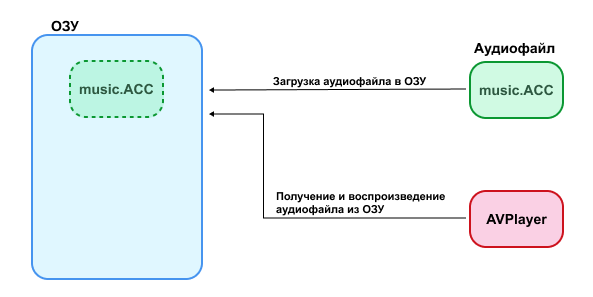
\includegraphics[scale=0.68]{img/AVPlayer-RAM.png}}
			\caption{Схема загрузки в оперативную память и воспроизведения аудиофайла с помощью AVPlayer.}
			\label{fig:avplayer-ram}
		\end{figure}

		\par Данный подход позволяет воспроизводить локальные аудиофайлы, хранящиеся на устройстве и имеющие формат ACC.
		Поддержка частоты дискретизации вплоть до 96 кГц, а также разрешение звука до 32 бит даёт возможность воспроизведения и управления
		аудиоданными высокого качества.

		\par В контексте воспроизведения потоковых аудиоданных необходим следующий сценарий использования AVPlayer:
		\begin{itemize}
			\item[1.] предварительное разбиение аудиофайла на подфайлы того же формата с определением метаинформации воспроизводимого участка базового файла на стороне сервера;
			\item[2.] поочерёдное получение и буферизация файлов (принцип очереди FIFO) на стороне клиента;
			\item[3.] поочерёдное получение и воспроизведение буферизованных файлов;
		\end{itemize}

		На рис. \ref{fig:avplayer-buffer} представлена схема буферизации подфайлов оригинального файла 
		и их перемещение в оперативную память для воспроизведения при потоковой передаче аудиоданных.

		\newpage
		\begin{figure}[!h]
			\center{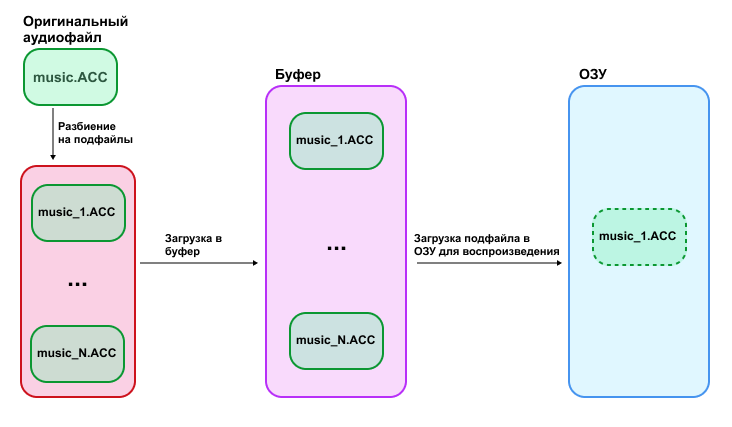
\includegraphics[scale=0.6]{img/AVPlayer-BUFFER.png}}
			\caption{Cхема буферизации подфайлов оригинального файла и их перемещение в оперативную память для воспроизведения при потоковой передаче аудиоданных.}
			\label{fig:avplayer-buffer}
		\end{figure}

		\par К плюсам данного подхода можно отнести:
		\begin{itemize}
			\item[---] поддержка аудиофайлов с частотой дискретизации до 96 кГц;
			\item[---] поддержка аудиофайлов с разрешеним звука до 32 бит;
		\end{itemize}

		\par К недостаткам данного подхода можно отнести:
		\begin{itemize}
			\item[---] полная выгрузка аудиоданных в оперативную память, отсутствие сегментации файла;
			\item[---] отсутствует системная поддержка потокового воспроизведения данных;
			\item[---] поддержка одного аудиоформата ACC;
			\item[---] дополнительные требования к стороне сервера для воспроизведения потоковых аудиоданных;
			\item[---] необходимость в реализации и поддержке буферизации файлов; 
		\end{itemize}

	\subsubsection{AVAudioPlayer}
		\par AVAudioPlayer \cite{avaudioplayer} --- программный интерфейс, являющийся частью комплекса программных интерфейсов AVFoundation.
		Он позволяет воспроизводить потоковые аудиоданные с помощью системного сегментатора.

		\par AVAudioPlayer поддерживает протокол потоковой передачи данных HLS, 
		частоту дискретизации до 48 кГц, а также разрешение звука до 16 бит.
		Основной особенностью является управление воспроизведением аудио.

		\par Системный сегментатор позволяет обрабатывать пакеты данных при потоковой передаче аудиоданных.
		Происходит обработка сегментов, сформированных протоколом потоковой передачи данных HLS,
		которая заключается в получении заголовка фрейма блока данных, который подаётся для воспроизведения.
		Использование сегментатора не позволяет накладывать звуковые эффекты на аудиопоток, 
		а также использовать системные вызовы для работы с аудиокартой.

		\par Для корректного воспроизведения потокового аудио с помощью программного интерфейса AVAudioPlayer,
		сторона сервера должна поддерживать передачу аудиоданных в формате ACC по протоколам семейства HLS.

		\par К плюсам данного подхода можно отнести:
		\begin{itemize}
			\item[---] системная поддержка потокового воспроизведение данных;
			\item[---] поддержка системного сигментатора; 
		\end{itemize}

		\par К недостаткам данного подхода можно отнести:
		\begin{itemize}
			\item[---] поддержка аудиофайлов с частотой дискретизации до 48 кГц;
			\item[---] поддержка аудиофайлов с разрешеним звука до 16 бит;
			\item[---] поддержка одного аудиоформата ACC;
			\item[---] дополнительные требовония к стороне сервера для воспроизведения потоковых аудиоданных; 
		\end{itemize}

	\subsubsection{AVAudioEngine}
		\par AVAudioEngine \cite{avengine} --- программный интерфейс, являющийся частью комплекса программных интерфейсов AVFoundation, 
		который поддерживает системные вызовы для взаимодействия с звуковой картой с помощью комплекса программных интерфейсов AudioToolbox.

		\par Работа с звуковой картой устройства \cite{coreaudio} поддерживает обработку пакетов аудиоданных для потокового воспроизведения, различные частоты дискретизации и разрешения звука, наложение звуковых эффектов,
		работу с нотной матрицей и обработку выделения памяти для хранения сегментов данных цифрового сигнала.
		При работе с аудиокартой необходимо реализовывать собственный сегментатор, так как системная поддержка стандартов протоколов потоковой передачи данных отсутствует.

		\par Принцип воспроизведения аудиоданных заключается 
		в поочерёдной обработке поступающего аудиосигнала с помощью создаваемых аудиоузлов, 
		которые изменяют звуковой сигнал заданным способом. Создаётся дерево связей аудиоузлов, 
		пройдя по которому на аудиосигнал наложатся звуковые эффекты или изменится метаинформация для воспроизведения аудиофайла.

		\par На рис. \ref{fig:avplayerengine-nodes} представлена схема прохождения аудиосигнала по дереву аудиоузлов.
		\begin{figure}[!h]
			\center{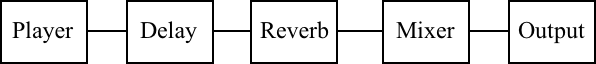
\includegraphics[scale=0.7]{img/AVPalyerEngine-nodes.png}}
			\caption{Схема прохождения аудиосигнала по дереву аудиоузлов.}
			\label{fig:avplayerengine-nodes}
		\end{figure}

		\par AVAudioEngine поддерживает хранение аудиосигнала в PCM формате, 
		т.к. на текущий момент он является стандартизированным решением.
		Работа с PCM форматом аудиосигнала достигается с помощью создания PCM буфера, 
		который позволяет хранить поступающие потоковое аудиоданные в виде потока байт.
		На рис. \ref{fig:AVPE-PCM-Buffer} представлена схема расположения фреймов аудиофайла в PCM буфере 
		для работы с AVAudioEngine.

		\newpage

		\begin{figure}[!h]
			\center{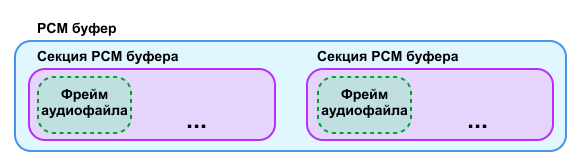
\includegraphics[scale=0.8]{img/AVPE-PCM-Buffer.png}}
			\caption{Схема расположения фреймов аудиофайла в PCM буфере.}
			\label{fig:AVPE-PCM-Buffer}
		\end{figure}

		\par Как подчёркивалось выше, AVAudioEngine поддерживает работу с системными вызовами 
		для обработки поступающего потока аудиоданных. Ниже приведены примеры некоторых из системных вызовов:
		\begin{itemize}
			\item[---] AudioFileStreamOpen --- открывает новый анализатор потока аудиоданных;
			\item[---] AudioFileStreamClose --- закрывает анализатор потока аудиоданных;
			\item[---] AudioFileStreamParseBytes --- передает данные потока аудиоданных анализатору;
			\item[---] AudioFileStreamGetPropertyInfo --- получение информации о текущем потоке аудиоданных; 
		\end{itemize}

		\par К плюсам данного подхода можно отнести:
		\begin{itemize}
			\item[---] поддержка потокового воспроизведения аудиоданных;
			\item[---] поддержка работы с системными вызовами;
			\item[---] поддержка PCM буфера; 
			\item[---] поддержка наложения звуковых эффектов;
			\item[---] поддержка различных частот дискретизации и разрешений звука;
		\end{itemize}

		\par К недостаткам данного подхода можно отнести:
		\begin{itemize}
			\item[---] отсутствие поддержки системного сегментатора;
		\end{itemize}

	\subsubsection{Сравнение средств воспроизведения аудиоданных в операционной системе iOS}
		\par Сравнение рассмотренных средств воспроизведения аудиоданных в операционной системе iOS рассмотрены в табл. \ref{tab:ios}. 
		Обозначения:
		\begin{itemize}
			\item[---] 1 --- поддержка частоты дискретизации более 48 кГц;
			\item[---] 2 --- поддержка воспроизведения потоковых данных;
			\item[---] 3 --- воспроизведение в режиме реального времени;
			\item[---] 4 --- наложение звуковых эффектов;
			\item[---] 5 --- наличие встроенного сегментатора для обработки потоковых данных;
			\item[---] 6 --- поддержка различных форматов аудиофайлов отличных от ACC;
			\item[---] 7 --- поддержка системных вызовов;  
			\item[---] 8 --- поддержка различных протоколов потоковой передачи данных;  
		\end{itemize}

		\begin{table}[hbtp]
			\caption{Сравнение средств воспроизведения аудиоданных в операционной системе iOS}
			\centering
			\label{tab:ios}
			\begin{tabular}{|p{150pt}|l|l|l|l|l|l|l|l|}
				\hline
				\textbf{Подход} & \textbf{1} & \textbf{2} & \textbf{3} & \textbf{4} & \textbf{5} & \textbf{6} & \textbf{7} & \textbf{8}  \\ \hline
				AVPlayer        & \textbf{+} & -          & -          & -          & -          & -          & -          & -           \\ \hline
				AVAudioPlayer   & -          & \textbf{+} & -          & -          & \textbf{+} & -          & -          & -           \\ \hline
				AVAudioEngine   & \textbf{+} & \textbf{+} & \textbf{+} & \textbf{+} & -          & \textbf{+} & \textbf{+} & \textbf{+}  \\ \hline
			\end{tabular}
		\end{table}

		\par По результатам сравнения можно сделать вывод,
		что для воспроизведения потокового аудио в мобильном приложении на операционной системе iOS 
		лучше всего подходит программный интерфейс AVAudioEngine. Данный программный интерфейс поддерживает все форматы аудиофайлов, 
		работу с системными вызовами для управления звуковым потоком, наложение звуковых эффектов, работу с PCM буфером,
		а также в отличии AVAudioPlayer (поддерживает только HLS) различные протоколы потоковой передачи данных, 
		но накладывает обязательство в реализации собственного сегментатора аудиопотока.

\subsection{Формализация постановки задачи}
	\par Основываясь на проведенном анализе предметной области, 
	задачу воспроизведения потокового аудио в мобильном приложении на операционной системе iOS
	можно сформулировать следующим образом: необходимо спроектировать программно-алгоритмический комплекс, 
	принимающий поток аудиоданных, которые буфиризируются в PCM формат. 
	
	\par В качестве программного интерфейса для обработки аудиосигнала и наложения звуковых эффектов целесообразно использовать AVAudioEngine.
	Для воспроизведения аудиосигнала осуществить работу с PCM буфером с помощью системных вызовов.
	Для получения аудиоданных с помощью сетевого запроса необходимо поддержать прикладной протокол HTTP.

\subsection*{Выводы}
	В аналитическом разделе был проведён анализ предметной области, 
	включающий в себя обзор существующих решений для воспроизведения потокового аудио в мобильном приложении на операционной системе iOS. 
	В ходе анализа была сформулирована задача разработки программно-алгоритмического комплекса,
	проанализированы существующие методы решения поставленной задачи и предложен вариант её решения.

\pagebreak


